\documentclass[letter, 11pt, twocolumn]{article}

\usepackage[utf8]{inputenc}
\usepackage[spanish]{babel}

\usepackage[left=0.75in,right=0.75in,top=0.75in,bottom=0.75in,columnsep=0.5in]{geometry}
\usepackage{graphicx}
\usepackage{float}
\usepackage{hyperref}

\usepackage{amsmath}
\numberwithin{equation}{section}

\usepackage{physics}

\usepackage{siunitx}
\DeclareSIUnit{\belmilliwatt}{Bm}
\DeclareSIUnit{\dBm}{\deci\belmilliwatt}
\DeclareSIUnit\lightyear{ly}
\usepackage{booktabs}
\usepackage{scrextend}
\def\tablename{Tabla}
\usepackage{stfloats}

% https://tex.stackexchange.com/questions/235783/listings-recognize-numbers-and-1e-3

\usepackage{xcolor}
\definecolor{maroon}{cmyk}{0, 0.87, 0.68, 0.32}
\definecolor{halfgray}{gray}{0.55}
\definecolor{ipython_frame}{RGB}{207, 207, 207}
\definecolor{ipython_bg}{RGB}{247, 247, 247}
\definecolor{ipython_red}{RGB}{186, 33, 33}
\definecolor{ipython_green}{RGB}{0, 128, 0}
\definecolor{ipython_cyan}{RGB}{64, 128, 128}
\definecolor{ipython_purple}{RGB}{170, 34, 255}

\usepackage{listings}
\renewcommand{\lstlistingname}{Código}
\lstset{
    breaklines=true,
    %
    extendedchars=true,
    literate=
    {á}{{\'a}}1 {é}{{\'e}}1 {í}{{\'i}}1 {ó}{{\'o}}1 {ú}{{\'u}}1
    {Á}{{\'A}}1 {É}{{\'E}}1 {Í}{{\'I}}1 {Ó}{{\'O}}1 {Ú}{{\'U}}1
    {à}{{\`a}}1 {è}{{\`e}}1 {ì}{{\`i}}1 {ò}{{\`o}}1 {ù}{{\`u}}1
    {À}{{\`A}}1 {È}{{\'E}}1 {Ì}{{\`I}}1 {Ò}{{\`O}}1 {Ù}{{\`U}}1
    {ä}{{\"a}}1 {ë}{{\"e}}1 {ï}{{\"i}}1 {ö}{{\"o}}1 {ü}{{\"u}}1
    {Ä}{{\"A}}1 {Ë}{{\"E}}1 {Ï}{{\"I}}1 {Ö}{{\"O}}1 {Ü}{{\"U}}1
    {â}{{\^a}}1 {ê}{{\^e}}1 {î}{{\^i}}1 {ô}{{\^o}}1 {û}{{\^u}}1
    {Â}{{\^A}}1 {Ê}{{\^E}}1 {Î}{{\^I}}1 {Ô}{{\^O}}1 {Û}{{\^U}}1
    {œ}{{\oe}}1 {Œ}{{\OE}}1 {æ}{{\ae}}1 {Æ}{{\AE}}1 {ß}{{\ss}}1
    {ç}{{\c c}}1 {Ç}{{\c C}}1 {ø}{{\o}}1 {å}{{\r a}}1 {Å}{{\r A}}1
    {€}{{\EUR}}1 {£}{{\pounds}}1
}

%%
%% Python definition (c) 1998 Michael Weber
%% Additional definitions (2013) Alexis Dimitriadis
%% modified by me (should not have empty lines)
%%
\lstdefinelanguage{iPython}{
    morekeywords={access,and,break,class,continue,def,del,elif,else,except,exec,finally,for,from,global,if,import,in,is,lambda,not,or,pass,print,raise,return,try,while},%
    %
    % Built-ins
    morekeywords=[2]{abs,all,any,basestring,bin,bool,bytearray,callable,chr,classmethod,cmp,compile,complex,delattr,dict,dir,divmod,enumerate,eval,execfile,file,filter,float,format,frozenset,getattr,globals,hasattr,hash,help,hex,id,input,int,isinstance,issubclass,iter,len,list,locals,long,map,max,memoryview,min,next,object,oct,open,ord,pow,property,range,raw_input,reduce,reload,repr,reversed,round,set,setattr,slice,sorted,staticmethod,str,sum,super,tuple,type,unichr,unicode,vars,xrange,zip,apply,buffer,coerce,intern},%
    %
    sensitive=true,%
    morecomment=[l]\#,%
    morestring=[b]',%
    morestring=[b]",%
    %
    morestring=[s]{'''}{'''},% used for documentation text (mulitiline strings)
    morestring=[s]{"""}{"""},% added by Philipp Matthias Hahn
    %
    morestring=[s]{r'}{'},% `raw' strings
    morestring=[s]{r"}{"},%
    morestring=[s]{r'''}{'''},%
    morestring=[s]{r"""}{"""},%
    morestring=[s]{u'}{'},% unicode strings
    morestring=[s]{u"}{"},%
    morestring=[s]{u'''}{'''},%
    morestring=[s]{u"""}{"""},%
    %
    % {replace}{replacement}{lenght of replace}
    % *{-}{-}{1} will not replace in comments and so on
    literate=
    {á}{{\'a}}1 {é}{{\'e}}1 {í}{{\'i}}1 {ó}{{\'o}}1 {ú}{{\'u}}1
    {Á}{{\'A}}1 {É}{{\'E}}1 {Í}{{\'I}}1 {Ó}{{\'O}}1 {Ú}{{\'U}}1
    {à}{{\`a}}1 {è}{{\`e}}1 {ì}{{\`i}}1 {ò}{{\`o}}1 {ù}{{\`u}}1
    {À}{{\`A}}1 {È}{{\'E}}1 {Ì}{{\`I}}1 {Ò}{{\`O}}1 {Ù}{{\`U}}1
    {ä}{{\"a}}1 {ë}{{\"e}}1 {ï}{{\"i}}1 {ö}{{\"o}}1 {ü}{{\"u}}1
    {Ä}{{\"A}}1 {Ë}{{\"E}}1 {Ï}{{\"I}}1 {Ö}{{\"O}}1 {Ü}{{\"U}}1
    {â}{{\^a}}1 {ê}{{\^e}}1 {î}{{\^i}}1 {ô}{{\^o}}1 {û}{{\^u}}1
    {Â}{{\^A}}1 {Ê}{{\^E}}1 {Î}{{\^I}}1 {Ô}{{\^O}}1 {Û}{{\^U}}1
    {œ}{{\oe}}1 {Œ}{{\OE}}1 {æ}{{\ae}}1 {Æ}{{\AE}}1 {ß}{{\ss}}1
    {ç}{{\c c}}1 {Ç}{{\c C}}1 {ø}{{\o}}1 {å}{{\r a}}1 {Å}{{\r A}}1
    {€}{{\EUR}}1 {£}{{\pounds}}1,
    %
    literate=
    *{+}{{{\color{ipython_purple}+}}}1
    {-}{{{\color{ipython_purple}-}}}1
    {*}{{{\color{ipython_purple}$^\ast$}}}1
    {/}{{{\color{ipython_purple}/}}}1
    {^}{{{\color{ipython_purple}\^{}}}}1
    {?}{{{\color{ipython_purple}?}}}1
    {!}{{{\color{ipython_purple}!}}}1
    {\%}{{{\color{ipython_purple}\%}}}1
    {<}{{{\color{ipython_purple}<}}}1
    {>}{{{\color{ipython_purple}>}}}1
    {|}{{{\color{ipython_purple}|}}}1
    {\&}{{{\color{ipython_purple}\&}}}1
    {~}{{{\color{ipython_purple}~}}}1
    %
    {==}{{{\color{ipython_purple}==}}}2
    {<=}{{{\color{ipython_purple}<=}}}2
    {>=}{{{\color{ipython_purple}>=}}}2
    %
    {+=}{{{+=}}}2
    {-=}{{{-=}}}2
    {*=}{{{$^\ast$=}}}2
    {/=}{{{/=}}}2,
    %
%   identifierstyle=\color{red}\ttfamily,
    commentstyle=\color{ipython_cyan}\ttfamily,
    stringstyle=\color{ipython_red}\ttfamily,
    keepspaces=true,
    showspaces=false,
    showstringspaces=false,
    %
    rulecolor=\color{ipython_frame},
    frame=single,
    frameround={t}{t}{t}{t},
    framexleftmargin=6mm,
    numbers=left,
    numberstyle=\tiny\color{halfgray},
    %
    %
    backgroundcolor=\color{ipython_bg},
    %   extendedchars=true,
    basicstyle=\scriptsize\ttfamily,
    keywordstyle=\color{ipython_green}\ttfamily,
    escapechar=\¢,escapebegin=\color{ipython_green},
}


\title{Informe Instrumentación Astronómica}
\author{Camilo Núñez Barra}


\begin{document}
\begin{figure}[H]
	
\includegraphics[width=2in]{fcfm_das}
\end{figure}
\begin{center}
	\textbf{\huge{INFORME\\INSTRUMENTACIÓN\\ASTRONÓMICA}}\\\,\\Tarea 1\\\,
\end{center}
\begin{tabular}{rl}
	Estudiante:&Camilo Núñez Barra\\
	RUT:&20.533.326-6\\
	Profesor:&Leonardo Bronfman\\
	Auxiliar:&Paulina Palma\\
	Curso:&AS3201 Astronomía Experimental\\
	Fecha:&\today
\end{tabular}

\section{Introducción}

\subsection{Motivación}

La emisión de radiación electromagnética ha permitido descubrir la composición, cinemática y distribución del medio intergaláctico y estrellas.

La nubes frías de hidrógeno gaseoso no emiten luz visible sino ondas de radio. Estas nubes son importantes porque pueden indicar el lugar de nacimiento de estrellas.

La radioastronomía usa radiotelescopios que captan ondas de radio, de longitudes de aproximadamente \SI{1}{\centi\meter} a \SI{10}{\meter}. Favorablemente, estas ondas coinciden con una ventana en la atmósfera, permitiendo su detección. A pesar de esto, la atmósfera sigue teniendo opacidad, dando lugar a errores en la medición de las señales, al igual que el error sistemático provocado por el instrumento mismo y su receptor en la antena.

Este informe trata sobre, primero, ciertas calibraciones para el radiotelescopio que permiten mejorar la precisión de las mediciones y, en segundo lugar, sobre el estudio de la nebulosa de Orión.

\subsection{Estructura del Informe}

La sección \ref{sec:radiotelescopio} introduce el radiotelescopio y la sección \ref{sec:mini} el radiotelescopio utilizando en este informe. Las secciones \ref{sec:hotcoldtest} y \ref{sec:antennadipping} tratan sobre dos calibraciones para el telescopio, el Hot--Cold Test y Antenna Dipping, respectivamente, incluyendo un marco teórico, presentación de los datos medidos y cálculo de calibraciones, junto con la comparación con respecto a las provistas por el software del radiotelescopio. La sección \ref{sec:observaciones} introduce el objeto celeste observado, junto con los espectros, temperatura de la fuente y errores asociados. Finalmente, la sección \ref{sec:conclusiones} presenta las conclusiones del informe y la sección \ref{sec:anexo} es un anexo con los códigos utilizados para los cálculos y gráficos.

\subsection{El radiotelescopio}\label{sec:radiotelescopio}

Un radiotelescopio es una antena especializada en captar ondas de radio. Generalmente tiene una antena parabólica, con un reflector principal que redirige la radiación recibida del cielo, concentrándola en un reflector secundario pequeño y contrapuesto, que a su vez redirige la señal concentrándola en un pequeño receptor en la bocina de la antena.

La potencia espectral $w$ recibida por unidad de ancho de banda es,
\begin{equation}
w=\frac{1}{2}A_\textnormal{e}\iint_\Omega{B(\theta,\phi)P_n(\theta,\phi)\dd{\Omega}}\label{eq:w}
	,\end{equation}
donde $A_\textnormal{e}$ es la apertura efectiva de la antena, $B$ es el brillo del cielo, $P_n$ es el patrón de potencia normalizado de la antena que mide de la respuesta de sus lóbulos como función de los ángulos, y $\dd{\Omega}$ es el elemento infinitesimal de ángulo sólido del cielo. Además, el factor $1/2$ es debido a que la antena es responsable de una sola componente de polarización de la radiación.

\subsection{Radiotelescopio MINI}\label{sec:mini}

Los experimentos de este informe se realizan gracias a las mediciones hechas por el equipo docente mediante el radiotelescopio Southern Millimeter-Wave Telescope (ver figura \ref{fig:mini}), que ha permitido importantes investigaciones como un mapeo extenso y uniforme del carbolo interestelar de toda nuestra galaxias. Actualmente se usa para observaciones docentes, como la de este curso e informe.

Este telescopio se denomina MINI por su pequeño tamaño. Está en su propio domo en el Observatorio Astronómico Nacional, en la cima del cerro Calán. Su antena tiene un diámetro de \SI{1.2}{\meter}. Tiene instalado un amplificador HEMT (High Electro Mobility Transistor) en la primera etapa de recepción que proporciona una mejor relación señal a ruido. Tiene dos espectrómetros de banco de filtros con 256 canales cada uno, que captan ondas electromagnéticas con frecuencias d \SI{86}{\giga\hertz} a \SI{115}{\giga\hertz}, con resoluciones respectivas de \SI{0.1}{\mega\hertz} y \SI{1}{\mega\hertz}.

\begin{figure}[p]
	\centering
	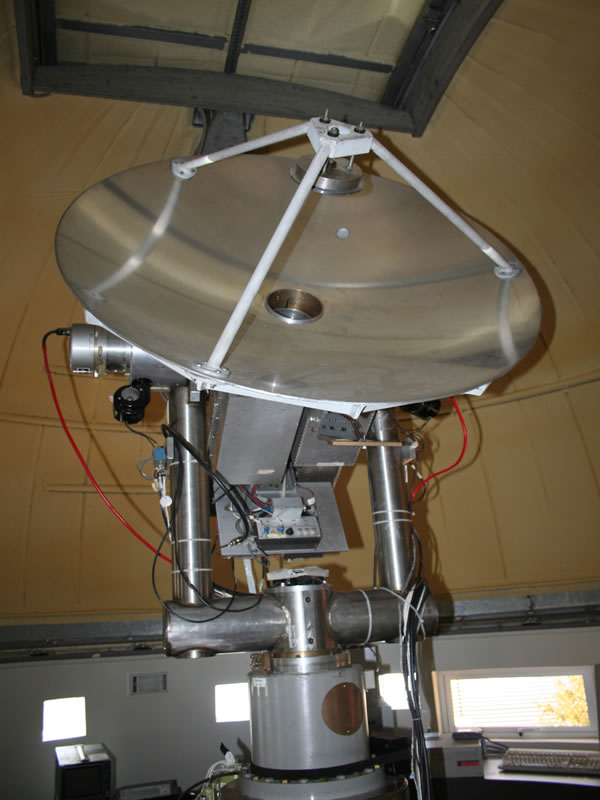
\includegraphics[width=3.25in]{mini.jpg}
	\caption{Radiotelescopio MINI (Imagen: DAS, FCFM)}
	\label{fig:mini}
\end{figure}

\begin{figure}[p]
	\centering
	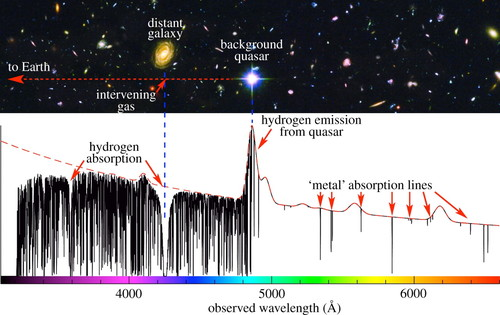
\includegraphics[width=3.25in]{spectrum.jpg}
	\caption{Espectro de absorción de un cuásar distante (Imagen: Joe Liske, ESO)}
	\label{fig:spectrum}
\end{figure}

\subsection{Espectros de absorción}

La potencia recibida (ecuación \ref{eq:w}) se puede recolectar a través de todos los canales del radiotelescopio, cada uno con una resolución determinada y un ancho de banda respectivo, permitiéndo graficarla en lo que se denomina espectro de absorción, como el que muestra la figura \ref{fig:spectrum}, que es para la luz visible pero sigue siendo ilustrativo para cualquiera. Las frecuencias o longitudes de ondas, adicionando su corrimiento debido al efecto Doppler, se pueden interpretar como velocidades radiales.

Una línea de absorción corresponde a un mínimo local preponderante en la curva del espectro y se producen porque los átomos en la línea de visión de la fuente se interponen en los fotones y absorben la energía para excitar sus electrones. Un ejemplo de absorción ocurre en las nubes de hidrógeno, que tienen temperaturas frías, y suelen indicar formación de estrellas.

Una línea de emisión corresponde a un máximo local preponderante en la curva del espectro y se produce por los fotones emitidos por las fuentes y los átomos que las componente. Un ejemplo de emisión ocurre en los cuásares y el hidrógeno que producen, estando a una muy alta temperatura.
\section{Hot--Cold Test}\label{sec:hotcoldtest}

\subsection{Marco teórico}

La señal de un objeto celeste recibida por un radiotelescopio se refleja en sus discos parabólicos para llegar al receptor espectrógrafo. El receptor tiene corrientes internas y fenómenos de transporte de electrones y fotones con ondas estacionarias que aumentan la entropía y generan también un error sistemático correspondiente a ruido blanco.

El ruido blanco del receptor se puede disminuir al aumentar el tiempo de integración pues la señal del cielo permanece constante y la señal del receptor disminuye relativamente su tamaño, por lo que disminuir el ruido permite disminuir el tiempo invertido para detectar una señal astronómica y a la vez permite no empeorar la señal.

Una manera común de eliminar errores sistemáticos es mediante la calibración del instrumento de medición.

El método Hot--Cold Test permite calibrar el telescopio al caracterizar la temperatura de ruido del receptor mediante dos cargas cuyas temperaturas son conocidas y diferentes.

Una carga es un material absorbente adherido a un pedazo de madera con un mango. El material es un absorbente electromagnético que absorbe la radiación con muy poca reflexión por lo que se supone como cuerpo negro. Si no fuera así, se formaría una onda estacionaria en la antena y las mediciones estarían fuertemente influidas por la posición de la carga.

Sea $T_\textnormal{rec}$ la temperatura de ruido del receptor y $G_\textnormal{rec}$ la ganancia del receptor. Una carga a temperatura ambiente $T_\textnormal{hot}$ se pone enfrente de la bocina de la antena, permitiendo medir una potencia espectral $W_\textnormal{hot}$ dada por,
\begin{equation}
W_\textnormal{hot}=G_\textnormal{rec}kT_\textnormal{rec}+G_\textnormal{rec}kT_\textnormal{hot}
,\end{equation}
donde $k$ es la constante de Boltzmann. Análogamente, para una carga fría a temperatura $T_\textnormal{cold}$, la potencia espectral medida es,
\begin{equation}
W_\textnormal{cold}=G_\textnormal{rec}kT_\textnormal{rec}+G_\textnormal{rec}kT_\textnormal{cold}
.\end{equation}
Se define el factor $Y$ como el cuociente entre la medición de la potencia espectral para la carga caliente y para la fría,
\begin{equation}
Y=\frac{W_\textnormal{hot}}{W_\textnormal{cold}}\label{eq:yfactor}
,\end{equation}
que permite determinar la temperatura de ruido del receptor mediante variables medidas,
\begin{equation}
T_\textnormal{rec}=\frac{T_\textnormal{hot}-YT_\textnormal{cold}}{Y-1}\label{eq:trec}
.\end{equation}

En términos de operación del telescopio, la medición de $T_\textnormal{rec}$ se hace cada día que es observa, por lo que en una campaña de meses se tiene que hacer todos los días la medición. Esta constante medición corresponde a un chequeo del estado de la electrónica del telescopio pues si repentinamente difiere mucho la temperatura de ruido del receptor con respecto a la medición del día anterior es porque está funcionando mal y se debe arreglar. En realidad se usa la potencia por canales de frecuencia y no la potencia espectral de todo el ancho de banda, tal como se describe en la sección \ref{sec:calibracion}, por lo que la temperatura de ruido del receptor cambia con la frecuencia.


\subsection{Datos y metodología}

Esta calibración utiliza una carga caliente a temperatura ambiente en la cúpula del radiotelescopio MINI y una carga fría a temperatura de nitrógeno líquido, cuyas mediciones están en la tabla \ref{tab:hotcoldtest}.

El MINI es pequeño, permitiendo acceder a la bocina por una escalera. Se sube y se pone la carga caliente enfrente de la bocina procurando apuntar el material absorbente a ella. Mediante un \textit{powermeter} se mide la potencia integrada de la señal para todo el ancho de banda que tiene el receptor y se anota la lectura en la tabla \ref{tab:hotcoldtest}.

A continuación y análogamente, se pone la carga fría enfrente de la bocina y se mide la potencia espectral con el \textit{powermeter} pero esperando a que la lectura correspondiente converja tras disminuir la temperatura. Esta medición está en la tabla \ref{tab:hotcoldtest}.

\begin{table}[p]
	\centering
	\begin{tabular}{
			@{}
			l
			S[table-format=3.0]
			S[table-format=2.2]
			@{}
		}
		\toprule
		{Carga} &
		{Temperatura} &
		{Potencia} \\
		{} &
		{\si{\kelvin}} &
		{\si{\dBm}} \\
		\midrule
		Hot & 300 & -44.50 \\
		Cold & 77 & -47.94 \\
		\bottomrule
	\end{tabular}
	\caption{Temperatura y potencia medidas para las cargas del Hot--Cold Test}\label{tab:hotcoldtest}
\end{table}

El \textit{powermeter} entrega potencias en decibelio-milivatio (\si{\dBm}), que es una escala logarítmica acorde a las eventuales amplificaciones y disminuciones de las señales. Una potencia $W$ en escala logarítmica de \si{\dBm} se convierte en una potencia $P$ en escala lineal de \si{\watt} como se muestra a continuación,
\begin{equation}
P=10^{\frac{W-3}{10}}\label{eq:dbm2w}
.\end{equation}

\subsection{Cálculo de $T_\textnormal{rec}$}

Se convierten las potencias de la tabla \ref{tab:hotcoldtest} a vatios según la ecuación \ref{eq:dbm2w} y se calcula $Y$ según la ecuación \ref{eq:yfactor}, obteniendo $Y=\num{2.2}$. Esto permite usar la ecuación \ref{eq:trec} para obtener $T_\textnormal{rec}=\SI{107.6}{\kelvin}$. Este cálculo se desarrolla en el código \ref{cod:hotcoldtest}.

\subsection{Comparación con calibración del MINI}\label{sec:calibracion}

El software del MINI tiene el comando \texttt{\%hct} para ingresar todo el sistema a una subrutina de Hot--Cold Test. Se usan cargas las mismas temperaturas de la tabla \ref{tab:hotcoldtest}.

El sistema espera a que se ponga la carga caliente en la bocina del receptor y se marca la medición al presionar una botonera, permitiendo tener una potencia por cada canal de frecuencia de la señal, mostrando una variación en todo el espectro. Ahora se pone la carga fría y se apreta la botonera, midiendo una potencia por cada canal que también varía en todo el espectro pero que es menor.

Se usan los dos vectores de potencia para calcular el factor Y según la ecuación \ref{eq:yfactor} y luego la temperatura de ruido del receptor por canal según la ecuación \ref{eq:trec}. Finalmente, se promedian las temperaturas de todos los canales, resultando una temperatura de ruido del receptor de $T_\textnormal{rec}'=\SI[separate-uncertainty=true]{150.9(46)}{\kelvin}$.

Se aprecia que $\abs{T_\textnormal{rec}'-T_\textnormal{rec}}=\SI{43.3}{\kelvin}$.
\section{Antenna Dipping}\label{sec:antennadipping}

\subsection{Marco teórico}

La turbulencias atmosféricas y el vapor de agua presente en la atmósfera distorsionan la señal de un objeto celeste dando lugar a un error sistemático que no depende del radiotelescopio.

La atmósfera en sus distintas capas varía la temperatura y la densidad pero en este experimento se hace una aproximación a primer orden para establecer que contribuye una temperatura de ruido $T_\textnormal{atm}$ fija. Además, se hace también una aproximación al igualar la temperatura ambiente del domo $T_\textnormal{amb}$ con $T_\textnormal{atm}$.

La opacidad cenital $\tau_\textnormal{w}$ debido al contenido de agua en la atmósfera y la opacidad cenital total $\tau_0$ de la atmósfera, que incluye al oxígeno, se aproximan también a primer orden para decir que son iguales.

El método Antenna Dipping permite calibrar el receptor del telescopio al determinar el estado y opacidad cenital de la atmósfera.

Se mide la potencia del cielo $W_\textnormal{sky}$ detectada por el telescopio a un determinado intervalo de frecuencias y elevación $\varphi$, que está dada por,
\begin{equation}
W_\textnormal{sky}=c\left(T_\textnormal{rec}+T_\textnormal{atm}\left(1-\exp\left(-\tau_\textnormal{0}/\sin\varphi\right)\right)\right)
,\end{equation}
donde $T_\textnormal{rec}$ es la temperatura de ruido del receptor y $c$ es una constante que, por ejemplo, puede depender de la ganancia del receptor.

Análogamente, la potencia para una carga enfrente de la bocina a temperatura ambiente $T_\textnormal{amb}$ (la misma carga Hot del Hot--Cold Test), la potencia es,
\begin{equation}
W_\textnormal{amb}=c\left(T_\textnormal{rec}+T_\textnormal{amb}\right)
.\end{equation}

Aplicando las aproximaciones, se define,
\begin{equation}
\Delta W\equiv W_\textnormal{amb}-W_\textnormal{sky}=cT_\textnormal{amb}\exp(-\tau_\textnormal{w}/\sin\varphi)\label{eq:deltaw}
,\end{equation}
y $z=\pi/2-\varphi$, permitiendo obtener la relación,
\begin{equation}
\ln\left(\Delta W\right)=-\sec\left(z\right)\tau_\textnormal{w}+\ln\left(cT_\textnormal{amb}\right)\label{eq:taufit}
,\end{equation}
que es una relación lineal de $\ln(\Delta W)$ con respecto a ${-\sec\left(z\right)}$, donde $\tau_\textnormal{w}$ es la pendiente de la recta.

\subsection{Datos y metodología}

Se utiliza una carga caliente a temperatura ambiente en la cúpula del radiotelescopio MINI, midiendo la potencia que muestra Domo en la tabla \ref{tab:taufit}.

Se mide con un \textit{powermeter} la potencia espectral de diez puntos a distintas elevaciones y azimut fijo, entregando los resultados de la tabla \ref{tab:taufit}.
\begin{table}[htbp]
	\centering
	\begin{tabular}{
			@{}
			l
			S[table-format=2.2]
			S[table-format=2.2]
			@{}
		}
		\toprule
		{Punto} &
		{Elevación} &
		{Potencia} \\
		{} &
		{\textdegree} &
		{\si{\dBm}} \\
		\midrule
		1 & 23.50 & -45.56 \\
		2 & 16.60 & -45.22 \\
		3 & 12.84 & -45.01 \\
		4 & 10.48 & -44.88 \\
		5 & 8.85 & -44.80 \\
		6 & 7.66 & -44.73 \\
		7 & 6.76 & -44.71 \\
		8 & 6.04 & -44.67 \\
		9 & 5.47 & -44.65 \\
		10 & 4.99 & -44.63 \\
		Domo & & -44.54 \\
		\bottomrule
	\end{tabular}
	\caption{Elevación y potencia para los distintos puntos a azimut fijo. Se incluye domo con carga caliente}\label{tab:taufit}
\end{table}

\subsection{Cálculo de $\tau_\textnormal{w}$}

El siguiente procedimiento corresponde al código \ref{cod:antennadipping}. Se lee el archivo \texttt{antdip\_AE2021A} provisto por el equipo docente con los datos necesarios para realizar el ajuste lineal según la ecuación \ref{eq:taufit}. El gráfico de este se muestra en la figura \ref{fig:taufit}. La pendiente de la recta establece un valor de \num{0.2573501} para la opacidad cenital debido al contenido de agua en la atmósfera.

\begin{figure}[htbp]
	\centering
	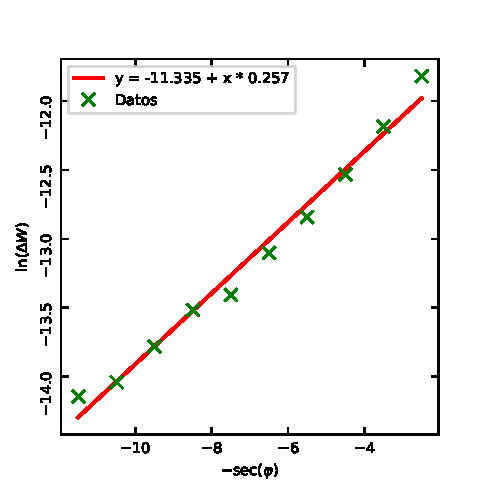
\includegraphics{taufit.pdf}
	\caption{Equis roja es medición del telescopio. Línea azul es ajuste lineal. La pendiente es $\tau_\textnormal{w}$}
	\label{fig:taufit}
\end{figure}

\subsection{Comparación con calibración del MINI}

El software del MINI tiene el comando \texttt{\%antdip} para ingresar todo el sistema a una subrutina de Antenna Dipping.

Primeramente se debe ingresar la cantidad de masas de aire por punto y se usa \num{1}, que es el valor típico.

Luego el sistema recolecta automáticamente información para diez puntos separados por una masa de aire a través de la elevación a azimut fijo, midiendo la mayor elevación primero y luego disminuye progresivamente. El telescopio constantemente evalúa su posición y solo toma datos cuando está apuntando con cierta tolerancia a la coordenada determinada por el sistema de control.

La información recolectada corresponde a la diferencia de potencia de la ecuación \ref{eq:deltaw}, donde la potencia para el cielo es la que apunta según la elevación correspondiente y la potencia para la carga caliente es según el \textit{chopper}, una carga absorbente electromagnética, que está dentro de la bocina de la antena y automática y periódicamente obstruye la visión del telescopio gracias a un motor.

Tras medir los diez puntos, automáticamente el telescopio apunta al domo y toma una medición de referencia con la carga caliente. A continuación, se debe ingresar la temperatura actual y la humedad relativa, además de un parámetro cualitativo de \num{0} a \num{3} que indica el grado de cobertura del cielo debido a las nubes y sirve para el registro histórico.

Finalmente, el software realiza el ajuste lineal y entrega el valor $\tau_\textnormal{w}'=\num{0.2573501}$, además de otros parámetros como la estimación de la eficiencia del telescopio y la temperatura de brillo del agua en el cielo.

Se aprecia que $\tau_\textnormal{w}=\tau_\textnormal{w}'$.
\section{Observaciones}

\subsection{Nebulosa de Orión}

Se observa la nebulosa de Orión (ver figura \ref{fig:m42}), también conocida como M42 por su identificación en el catálogo Messier. Esta es una nebulosa difusa situada al sur del cinturón de Orión (ver figura \ref{fig:lb}).
La nebulosa de Orión, también conocida como Messier 42, M42, o NGC 1976, es una nebulosa difusa situada al sur del cinturón de Orión. Tiene un radio de \SI{1.2}{\lightyear} y su distancia a la Tierra es de \SI{1344}{\lightyear}, por lo que es muy cercana y eso la convierte en una buena referencia. Además, en ella hay formación de estrellas de alta masa y también variadas moléculas y partículas, encontrando sus abundancias en \textit{surveys}.

\begin{figure}[p]
	\centering
	\includegraphics[width=3.25in]{m42.jpg}
	\caption{Nebulosa de Orión (Imagen: NASA)}
	\label{fig:m42}
\end{figure}

\begin{figure}[p]
	\centering
	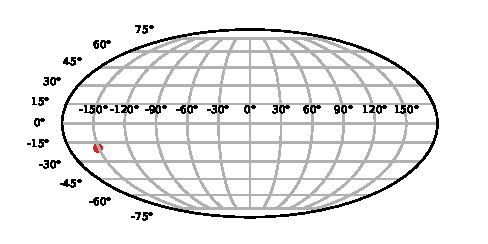
\includegraphics{lb.pdf}
	\caption{Coordenadas galácticas de la nebulosa de Orión}
	\label{fig:lb}
\end{figure}

Antes de la observación se hace la calibración del telescopio mediante el Hot--Cold Test y Antenna Dipping, tal como se explican en las secciones \ref{sec:hotcoldtest} y \ref{sec:antennadipping}, respectivamente. Esto es importante para tener observaciones más precisas.

Se hace una cruz en el cielo alrededor y centrada en la fuente, tal como muestra la figura \ref{fig:cruz}. Se apunta en el siguiente orden respecto a la figura: arriba, izquierda, centro, derecha y abajo. Esto se repite consecutivamente para un total de 3 pasadas a la cruz.

Los siguientes parámetros se establecen en el software del MINI.

Se usa el modo observacional \textit{position switching}, que necesita definir los puntos: \textit{on pos}, la posición de la fuente; \textit{off pos}, una posición de referencia y; \textit{home pos}, un punto central del mapa que es necesario para calcular la grilla.

Se usa la coordenada ecuatorial de la nebulosa de Orión RA=\ra{5;32;47} y DEC=\ang{-5;24;30} para \textit{on pos} y \textit{home pos}, mientras que para \textit{off pos} se usa RA=\ra{5;40;47} y DEC=\ang{-5;10;0}.

El ciclo \textit{on--off} es de \SI{30}{\second} en total y \SI{15}{\second} por cada posición

El tiempo de integración es \SI{600}{\second}, por lo que el tiempo de observación es el doble.

Además, constantemente se asigna un tiempo de calibración de \SI{5}{\second} para chequear que la atmósfera no ha cambiado respecto al modelo. El espectro obtenido se normaliza al continuo.

\begin{figure}[p]
	\centering
	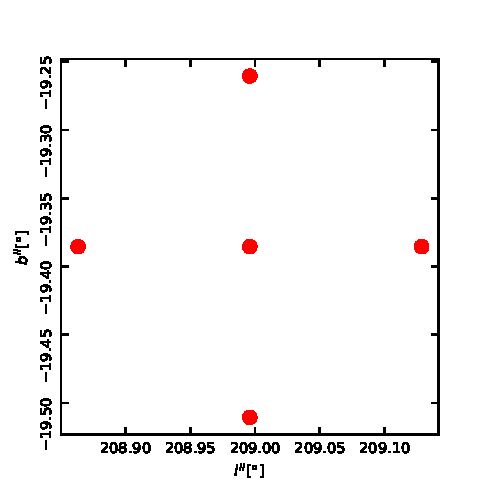
\includegraphics{cruz.pdf}
	\caption{Cruz de observación}
	\label{fig:cruz}
\end{figure}

El procedimiento para el análisis de las observaciones se muestra en el código \ref{cod:observaciones} y se detalla a continuación.

\subsection{Espectros}

La observación registra los datos provistos por el equipo docente en los archivos \texttt{sdf\_1xx\_1xx}, donde \texttt{xx} va en orden creciente \texttt{11} a \texttt{25}, según el orden de observación de la cruz explicado anteriormente. 

Se miden 256 temperatura en kelvin a distintas velocidades, formando un espectro con una preponderante línea de emisión aproximadamente \SI{9.5}{\kilo\meter\per\second} a aproximadamente \SI{30}{\kelvin} para el punto central. Se hace un ajuste gaussiano para cada uno de estos espectros y se grafica en las figuras \ref{fig:specfit1}, \ref{fig:specfit2} y \ref{fig:specfit3}, para la primera, segunda y tercera pasada por la cruz, respectivamente.

\begin{figure}[p]
	\centering
	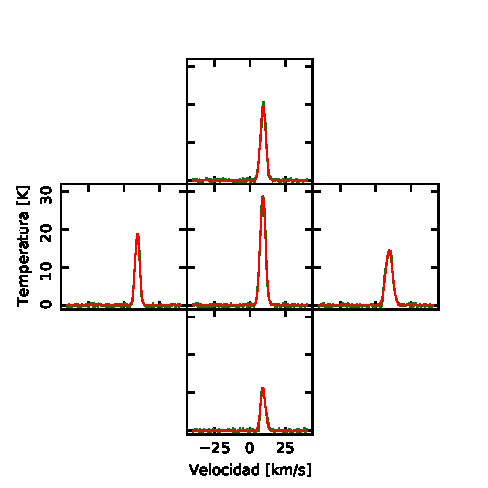
\includegraphics{specfit1.pdf}
	\caption{Gráfico del espectro y su ajuste gaussiano, primera pasada por la cruz. Línea verde es espectro original. Línea roja es ajuste.}
	\label{fig:specfit1}
\end{figure}

\begin{figure}[p]
	\centering
	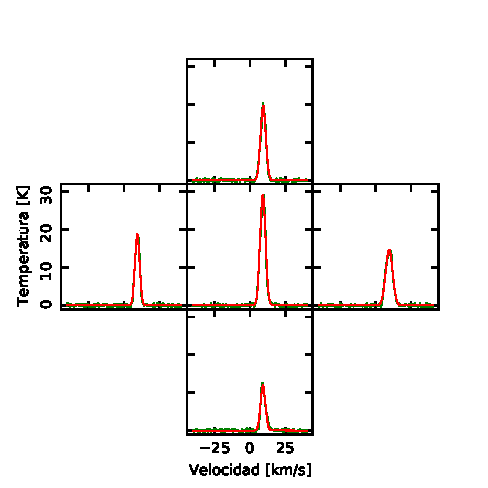
\includegraphics{specfit2.pdf}
	\caption{Gráfico del espectro y su ajuste gaussiano, segunda pasada por la cruz. Línea verde es espectro original. Línea roja es ajuste.}
	\label{fig:specfit2}
\end{figure}

\begin{figure}[p]
	\centering
	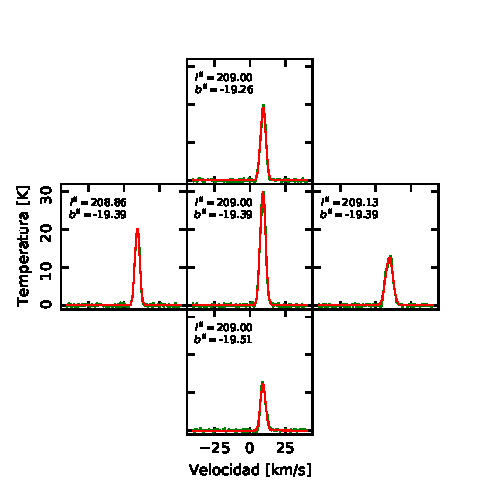
\includegraphics{specfit3.pdf}
	\caption{Gráfico del espectro y su ajuste gaussiano, tercera pasada por la cruz. Línea verde es espectro original. Línea roja es ajuste.}
	\label{fig:specfit3}
\end{figure}

\subsection{Temperatura máxima y Pointing}

Se calcula la temperatura máxima del espectro para cada una de las quince observaciones. Se promedian las temperaturas correspondientes a las mismas coordenadas en la cruz y se realizan dos ajustes gaussianos, tal como muestra la figura \ref{fig:tmax}. El primer ajuste es a través de la longitud galáctica, manteniendo la latitud galáctica fija, es decir, sobre los tres puntos horizontales de la cruz. El segundo ajuste es a través de la latitud galáctica, manteniendo la longitud galáctica fija, es decir, sobre los tres puntos verticales de la cruz.

\begin{figure}[p]
	\centering
	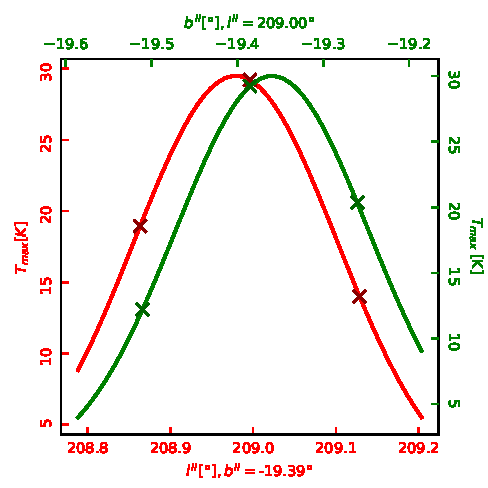
\includegraphics{tmax.pdf}
	\caption{Gráfico de temperatura máxima y su ajuste gaussiano. Línea roja es ajuste de los puntos a latitud fija y se mide en los ejes inferior e izquierdo. Línea verde es ajuste de los puntos a longitud fija y se mide en los ejes superior y derecho. Equis roja es medición en la cruz, en orden creciente de longitud: punto de arriba, centro y abajo. Equis verde es medición en la cruz, en orden creciente de latitud: punto de izquierda, centro y derecha.}
	\label{fig:tmax}
\end{figure}

El punto central de la cruz tiene una temperatura máxima de \SI{29.215}{\kelvin} a longitud galáctica \SI{208.006}{\degree} y latitud galáctica \SI{-19.385}{\degree}, mientras que el modelo del ajuste gaussiano a latitud fija establece un máximo de \SI{29.485}{\kelvin} a longitud \SI{208.975}{\degree} y el ajuste gaussiano a longitud fija establece un máximo de \SI{29.989}{\kelvin} a latitud \SI{-19.357}{\degree}.

Los datos anteriores muestra que el pointing del telescopio es aceptable, pues no hay diferencias de más de una unidad. A pesar de que el telescopio tenía ordenado apuntar a la coordenada precisa de la nebulosa de Orión, existe un error que se puede calibrar. Además, el software del telescopio tiene una ventana de tracking que muestra que tiene permitido apuntar dentro de un radio de tolerancia de la coordenada objetivo.

\subsection{Temperatura integrada}

Se calcula la temperatura integrada del espectro para cada una de las quince observaciones. Se promedian las temperaturas correspondientes a las mismas coordenadas en la cruz y se realizan dos ajustes gaussianos, tal como muestra la figura \ref{fig:tmax}. El primer ajuste es a través de la longitud galáctica, manteniendo la latitud galáctica fija, es decir, sobre los tres puntos horizontales de la cruz. El segundo ajuste es a través de la latitud galáctica, manteniendo la longitud galáctica fija, es decir, sobre los tres puntos verticales de la cruz.

\begin{figure}[p]
	\centering
	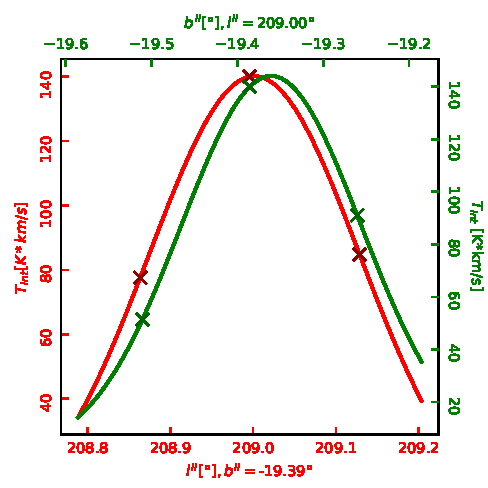
\includegraphics{tint.pdf}
	\caption{Gráfico de temperatura integrada y su ajuste gaussiano. Línea roja es ajuste de los puntos a latitud fija y se mide en los ejes inferior e izquierdo. Línea verde es ajuste de los puntos a longitud fija y se mide en los ejes superior y derecho. Equis roja es medición en la cruz, en orden creciente de longitud: punto de arriba, centro y abajo. Equis verde es medición en la cruz, en orden creciente de latitud: punto de izquierda, centro y derecha.}
	\label{fig:tint}
\end{figure}

\subsection{Error RMS y comparación}

Sea $\Delta T_\textnormal{A}$ el error total para $N$ muestras promediadas, $T_\textnormal{sys}$ el error para una única muestra, $\tau$ el tiempo total, $\Delta\nu$ el ancho de banda. La estadística gaussiana establece la siguiente relación entre el error para las muestras promediadas y el error para una única muestra,
\begin{equation}
\Delta T_\textnormal{A}=\frac{T_\textnormal{sys}}{\sqrt{N}}=\frac{T_\textnormal{sys}}{\sqrt{\tau\Delta\nu}}\label{eq:rms}
,\end{equation}
pero en la práctica hay un factor $C_\textnormal{obs}$ que depende del modo de observación,
\begin{equation}
\Delta T_\textnormal{A}=\frac{C_\textnormal{obs}T_\textnormal{sys}}{\sqrt{N}}=\frac{C_\textnormal{obs}T_\textnormal{sys}}{\sqrt{\tau\Delta\nu}}\label{eq:rms}
,\end{equation}
donde la constante observacional $C_\textnormal{obs}$ para el modo \textit{position switching}, que apunta tanto a la fuente como fuera de esta, es igual a $\sqrt{2}$.

Por un lado, se utiliza la técnica de \textit{sigma clipping} para obtener la base de ruido de los espectros y eliminar la línea de emisión para el siguiente cálculo, utilizando $\sigma=3$ y las iteraciones necesarias hasta que el algoritmo converja. Se calcula el error RMS del ruido para cada uno de los quince espectros.

Por otro lado, se promedian los espectros correspondientes a la misma coordenada en la cruz. Se les aplica la técnica de \textit{sigma clipping} con los mismos parámetros anteriores. Se calcula el error RMS del ruido para cada uno de los cinco nuevos espectros.

Los resultados se muestran en la tabla \ref{tab:rms}, que tiene los valores $\Delta T_\textnormal{A}/T_\textnormal{sys}$.

La ecuación \ref{eq:rms} y la cantidad de datos promediados establecen que el cuociente teórico entre el error del promedio y el error de una muestra única es $1/\sqrt{3}=0.577$, pero si se considera la constante observacional entonces es $\sqrt{2}/\sqrt{3}=0.816$.

\begin{table*}[htbp]
	\centering
	\begin{tabular}{
			@{}
			l
			S[table-format=2.3]
			S[table-format=2.3]
			S[table-format=2.3]
			S[table-format=2.3]
			S[table-format=2.3]
			@{}
		}
		\toprule
		{Pasada} &
		{Arriba} &
		{Izquierda} &
		{Centro} &
		{Derecha} &
		{Abajo} \\
		\midrule
		Primera & 0.583 & 0.573 & 0.579 & 0.555 & 0.552 \\
		Segunda & 0.621 & 0.601 & 0.640 & 0.628 & 0.593 \\
		Tercera & 0.637 & 0.619 & 0.626 & 1.084 & 0.599 \\
		\bottomrule
	\end{tabular}
	\caption{Cociente entre error de los puntos de la cruz promediados y error de los puntos sin promediar}\label{tab:rms}
\end{table*}


\section{Conclusiones}
\onecolumn

\section{Anexo}

\lstinputlisting[language=iPython, label={cod:hotcoldtest}, caption={Hot--Cold Test}]{anexos/hotcoldtest.py}

\lstinputlisting[language=iPython, label={cod:antennadipping}, caption={Antenna Dipping}]{anexos/antennadipping.py}

\lstinputlisting[language=iPython, label={cod:observaciones}, caption={Observaciones}]{anexos/observaciones.py}

\end{document}